\chapter{Curation and Administration}
\index{Curation|(}


\section{Laboratory workflow}
\index{Workflow}
Corina includes a number of functions to assist you with the curation of your physical sample collection.  To understand how these are designed to assist users, we must first consider the workflow within a laboratory.

In research laboratories, samples generally come to the lab in large batches following field collection.   In this case the typical workflow may be as follows:

\begin{enumerate*}
 \item Collect samples and record field notes as accurately as possible
 \item On returning to the lab enter field notes as soon as possible into the `bulk data entry' interface
 \item Print sample barcode labels
 \item Prepare physical samples and label with barcodes
 \item Assign samples to storage boxes
 \item Measure samples, using barcodes to recall metadata from database
 \item Crossdate samples / build chronologies
 \item When all samples from a box are completed register box as archived and then store
\end{enumerate*}

For commercial labs offering dendrochronological dating as a service, samples more likely to arrive in smaller batches.  In this case, the bulk data entry interface may not be the most efficient method for entering metadata.  In this case the user may simply prefer to use the \menutwo{File}{New} method for each sample.  

Either way, the concept behind the curation of a collection in Corina revolves around the accurately recording as much metadata about a sample as possible, then labeling the physical sample with a label containing a barcode for Corina and sample code for the user.  By entering a sample into the database as soon as it enters the lab, it can be traced throughout the workflow.  When a chronology is built, it is easily to quickly and efficient locate all samples that have been used.  By assigning samples to boxes, groups of similar samples (e.g.\ from the same site) can also be easily stored together and located quickly and efficiently.  


\section{Barcodes}
\label{txt:barcodes}
\index{Barcodes}

Barcodes allow you to keep track of what samples you have and where they are stored.  Although it is not essential to use the barcode functions, we strongly suggest you do because they save time and money, but most importantly they greatly reduce the scope for erroneous data entry.  For instance, when measuring a sample a user simply scans its barcode and all the relevant metadata is retrieved from the database, rather than relying on them to enter data manually.  Barcodes have been routinely used in the retail industry since the 1980s.  They can be equally as useful in dendrochronology laboratories.

Corina creates and reads barcodes for samples, measurement series and boxes.  Each barcode encodes the unique identification code stored in the Corina database for each of these entities.  Due to Corina's use of universally unique identifiers (UUIDs), these codes are guaranteed to be unique opening the opportunity of labs to loan samples, much like libraries do with books.  There are many styles (or `symbologies') of barcodes in use today, but Corina uses one of the most common (Code 128) which is supported by the vast majority of barcode readers.  For a detailed discussion on the specifications of the Corina barcode see section \ref{txt:barcodeSpecs}.

Basic barcode readers are now cheap and widely available, with basic devices retailing for a few tens of dollars.  Most are characterized as `keyboard interface devices' and work like an automated keyboard, typing in a string of characters when a label is scanned.  

Within the Corina application, whenever the user is required to specify a box, sample or series, they have the option of typing the human readable lab code or scanning the barcode. By using the barcode, the user can be sure they are not entering typographic errors so we recommend using barcodes whenever possible. 

The most important barcode is the label for the physical wood sample.  These are easily generated through the \menuthree{Administration}{Labels}{Sample labels} menu entry.  Currently the layout of these labels is fixed, but in the future we aim to provide different styles.  

\subsection{Sample labels}
\index{Labels!Samples}
Before labels can be generated, metadata entries the sample level must have been made in the database.  This is typically done using the `bulk data entry' interface (see page \pageref{txt:bulkentry}).  If samples are already in the database, the user needs to select the object of interest in the label creation dialog to see all the available samples.  It is then just a matter of selecting the samples of interest and moving them into the `selected' column.  Once the list is populated (samples from multiple objects can be included), then you can either click `Preview' to see a PDF of the labels, or `Print' to print directly.

\begin{figure}[hbtp]
  \centering
    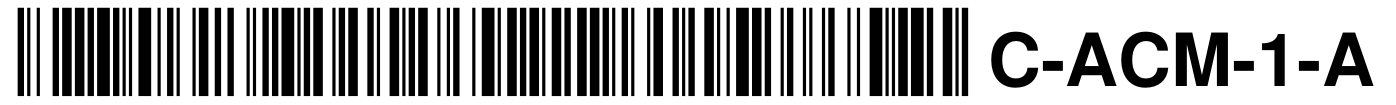
\includegraphics[width=100mm]{Images/samplebarcode.png}
    \caption{An example of a sample barcode produced by Corina for the Cornell lab.  Note the label also includes the human readable code for the sample.}
    \label{fig:graph}
\end{figure}

The current label style is designed to fit on standard core mounts and most samples.  There are no widely available die-cut labels that fulfill this need, so the labels are intended to be printed on archival grade full page sheet labels (e.g.\ Avery\textsuperscript{\textregistered} layout 6575), and then manually guillotined.  

\subsection{Box labels}
\index{Labels!Boxes}
The procedure for printing box labels is the same as for samples.  Samples must have already been assigned to boxes before the label is printed (see section \ref{txt:assignToBox} for details).  To print (or preview) box labels go to \menuthree{Administration}{Labels}{Box labels}.  The label style is designed to be printed on $5'' \times 8{1 \over 8}''$ labels, two per sheet such as the Avery\textsuperscript{\textregistered} 6579 layout.  An example is shown in figure \ref{fig:boxlabel}.

\begin{figure}[htbp]
  \centering
    \setlength\fboxsep{0pt}
    \setlength\fboxrule{0.5pt}
    \fbox{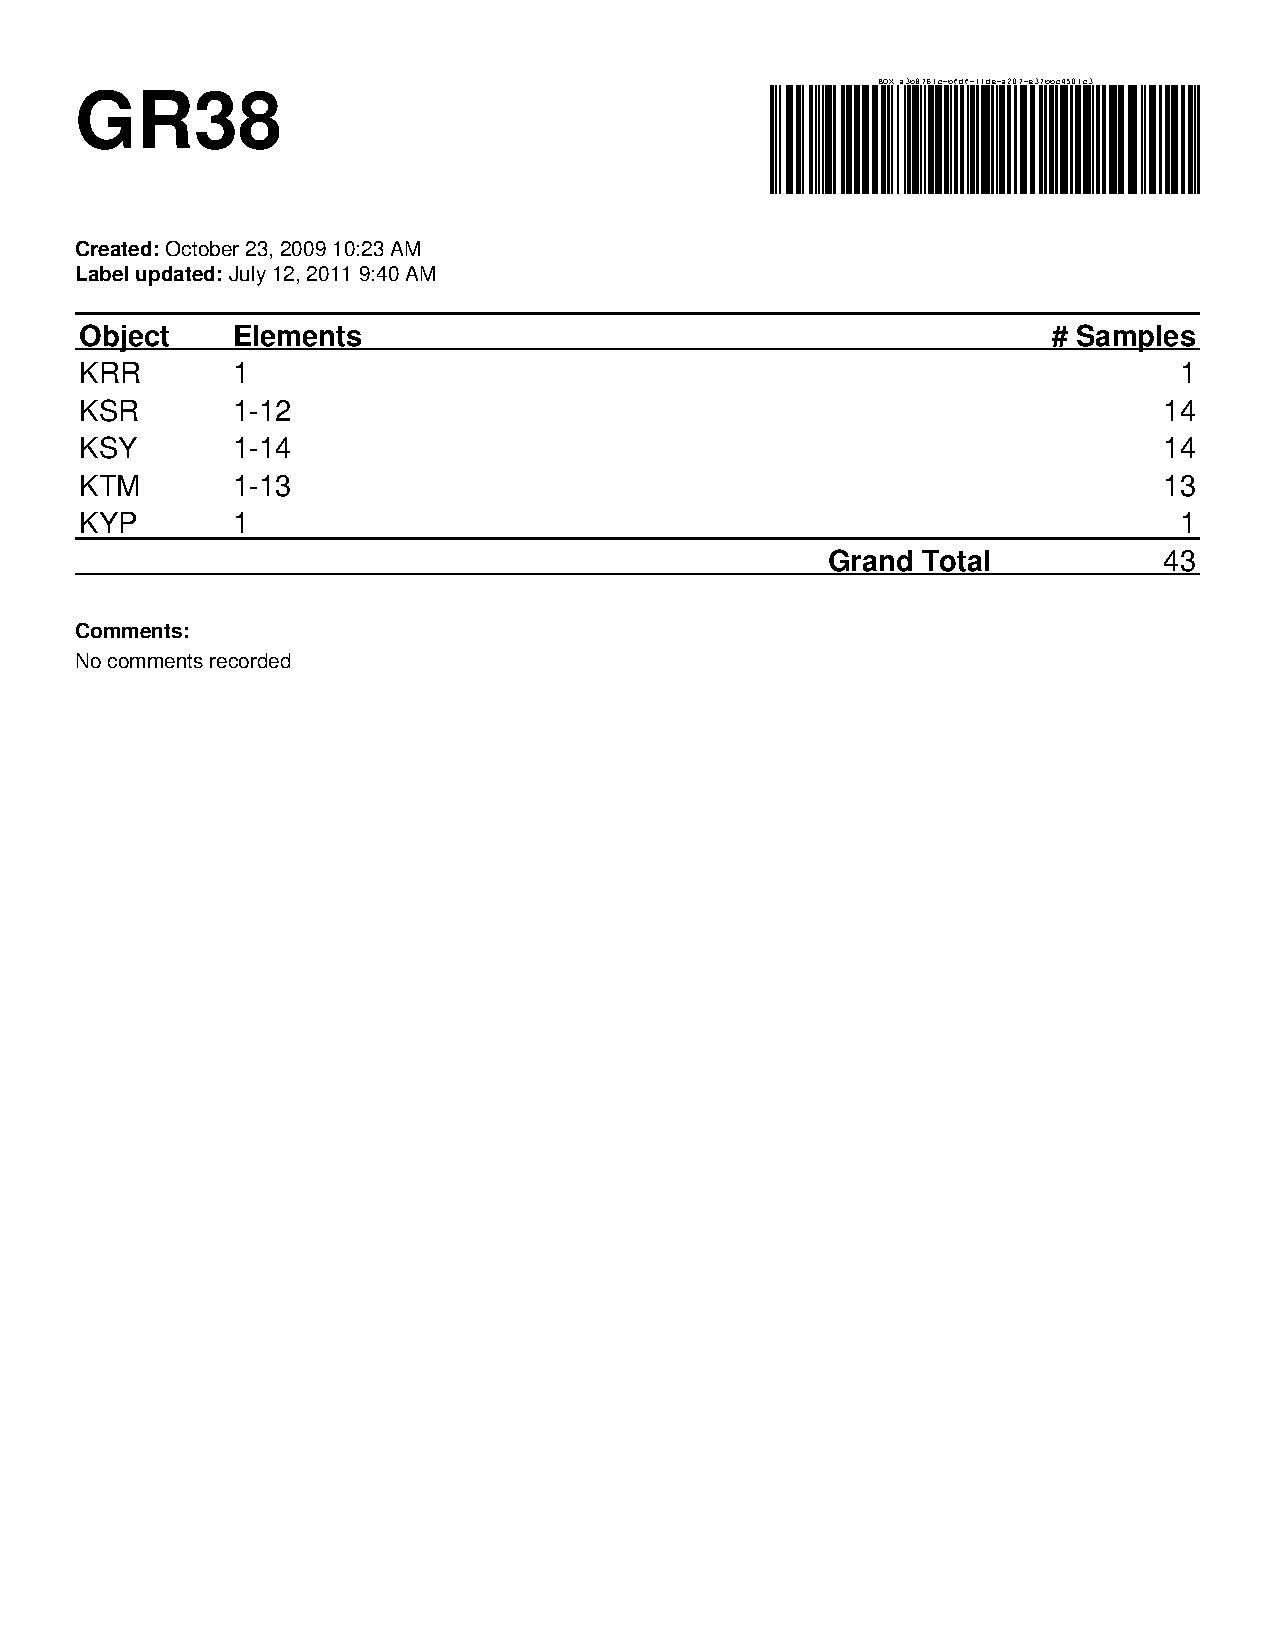
\includegraphics[width=\textwidth, trim=0 15cm 0 0]{Images/boxlabel.pdf}}
    \caption{An example of a box label from the Cornell collection. The label provides a human readable name for the box (GR38), a barcode for accessing the box details within Corina, and a summary of the samples contained within the box.}
    \label{fig:boxlabel}
\end{figure}

\info{Until dynamic label styles have been implemented, box labels will print one per page.  To make use of the second label on the page, the same sheet should be fed through the printer a second time.}

\subsection{Series barcodes}

Series barcodes are printed at the top of a standard series report (see figure \ref{fig:seriesreport}).  These are produced through the \menutwo{File}{Print}, or \menutwo{File}{Print preview}, menus.  

\begin{figure}[p]
  \centering
    \setlength\fboxsep{0pt}
    \setlength\fboxrule{0.5pt}
    \fbox{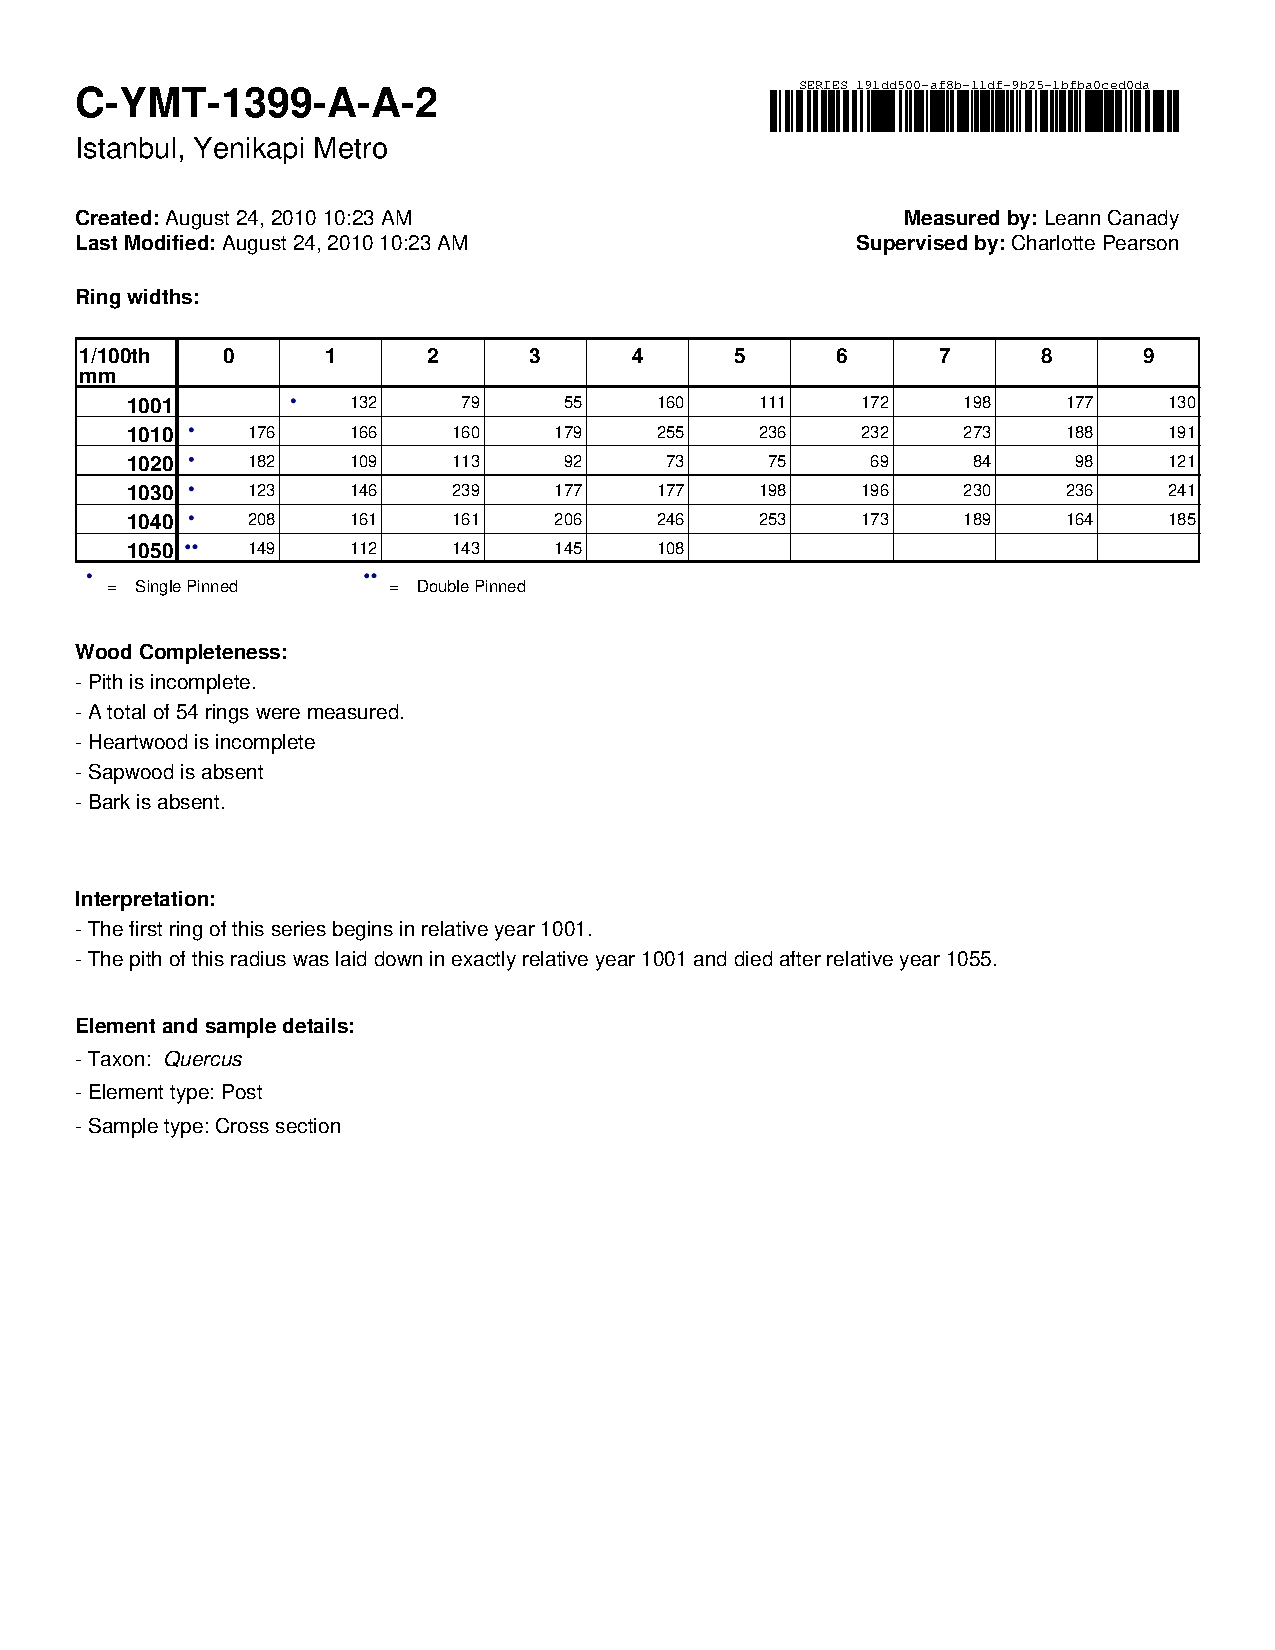
\includegraphics[width=\textwidth]{Images/seriesreport.pdf}}
    \caption{An example of a report showing barcode and basic metadata about a series.  }
    \label{fig:seriesreport}
\end{figure}


\section{Storage boxes}
\label{txt:assignToBox}
\index{Boxes}
Corina uses the term `box' to refer to the collection of samples you archive.  Many labs (including Cornell) use cardboard bankers boxes to store samples once they are completed, but the same box concept could refer to draws or shelves in your collection.

\subsection{Creating and editing boxes}
\index{Boxes!Creating}
\index{Boxes!Editing}
Records for boxes in the system are created and edited through the \menuthree{Administration}{Curation}{Box details} menu.  To editing an existing box, you can scan the barcode label on the box, or select from the list.  To create a new box, click the `Create new box' button and enter its details.  There is no restriction on what boxes should be called, but it is probably easiest if you use some sort of numerical sequence to assist with organizing the boxes in your store.  At Cornell, we use a two part name for each, the first being the year of collection, the second being a sequential number (e.g.\ 2009-11).

\index{Sample!Assign to box}The contents tab lists all the samples that have been assigned to this box.  To add new samples, simply click the `Add sample to box' button and scan the sample's barcode.  

\subsection{Inventory}
\index{Inventory}
An important feature of any collection management system is the ability to perform an inventory on the collection.  Even with the most robust system, samples will always go astray so its important to be able to periodically check that the boxes contain what you expect.

The `Contents' tab of the Box details dialog contains a feature to assist with this.  Next to the list of samples that are recorded as present, there is a temporary checklist column.  By checking the boxes for each sample actually stored in the box it is easy to see which samples have been mislaid.  If the `Mark unchecked as missing from box' button is then pressed, the date and time the discrepancy was noted is then recorded in the comments field for the box.

\subsection{Checking boxes in and out}
\index{Boxes!Checking in and out}
Corina includes function for checking boxes in and out of a store, much like when a book is borrowed from a library.  The \menuthree{Administration}{Curation}{Check out box from store} and \menuthree{Administration}{Curation}{Return box to store} menus do just this.  You can either scan the box barcode or select the box from the drop down menu.  These options record when a box is checked out/in and by whom.  These details can be seen by users in the box details dialog.

\subsection{Locating samples}
\index{Sample!Locating}
As you might expect, Corina also includes a function for locating your physical samples.  This is available in the \menuthree{Administration}{Curation}{Find a sample} menu.  There are three methods for locating a sample: via barcode; via lab code; and manually by object/element/sample.  

If you have the sample in your hand and you simply want to know which box it should be returned to you can scan the barcode.  If you are looking for a sample and you know its lab code then you can enter this instead.  Alternatively, you can use the drop down menus to search for one or more samples at once.  For instance, you can locate all the samples for a particular object and element.


\index{Curation|)}